\chapter{Implementation Details}
\label{chap:implementation}
This chapter explains several technical implementation details. The first section describes span exporters and API of Trace Context. The following section focuses on implementation details of the native agent and the last section focuses on the implementation details of the instrumentation server.

\section{Span and Trace Trees}
This section explains two implementation specific areas related to spans and trace trees. It describes span exporters in more detail and gives an overview of the Trace Context API. 
\subsection{Span Exporters}
\label{imp:exporter}
Implementation of span exporters have to extend from the abstract ancestor defining common methods for each span exporter. Also, in order to be able to use the exporter automatically in the code, it has to have a constructor with single \texttt{String} argument accepting exporter arguments. The arguments format is defined in the case of default span exporters, however the developer may use any format in case of custom span exporters. \texttt{SpanExporter} abstract class is the common ancestor for each exporter and has two abstract methods:
\begin{itemize}
	\item \texttt{export}. This method is used for exporting the span. Custom span exporters implementation may save the data on local disk or send over network. The destination is not limited by the code. Internally, the \texttt{export} method is called asynchronously in separated threads to allow asynchronous span exporting, which can lead to a performance benefit.
	\item \texttt{parseAndSetArgs}. The native agent has configuration property, which the user can use to configure arguments for the span exporter. Each span exporter is responsible for parsing its own arguments.
\end{itemize}

As mentioned in the Section \ref{design:exporter}, the Distrace tool provides two default implementations of span exporters:
\begin{itemize}
	\item  \texttt{DirectZipkinExporter} -  This span exporter sends the collected span asynchronously to the user interface right away without storing the data on disk to be collected by any data collection agent. In this case, the functionality of the span exporter and the data collector are handled by this single exporter.
	This span exporter should be used only for demonstration purposes, since it could overload the user interface or network when processing high number of spans, because the Zipkin user interface is not prepared to handle and store large amount of data in the memory. However, this is a default span exporter at this moment.
	
	This exporter accepts a single argument, which is the IP address and port of the Zipkin user interface. The Figure \ref{fig:zipkin_span_exporter} shows, how the Zipkin span exporter is used.
	
	\begin{figure}
		\centering
		
\includegraphics[scale=0.6]{zipkin_span_exporter.png}
		\caption{Using the Zipkin span exporter to export spans directly to Zipkin user interface without the data collection agent.}
		\label{fig:zipkin_span_exporter}
	\end{figure}
	\item  \texttt{JSONDiskExporter} - The second available span exporter saves the collected spans asynchronously on disk in the format known to the Zipkin user interface. The exported spans may be collected in the future by a custom data collection agent and for example, sent to the user interface or database. Together with some well-known data collection agent, this is a preferred way of transferring spans from the application to the Zipkin user interface in the production. This exporter accepts single argument, which is a destination directory for exported spans. The Figure \ref{fig:disk_span_exporter} shows how JSON disk span exporter is used.
	\begin{figure}
		\centering
		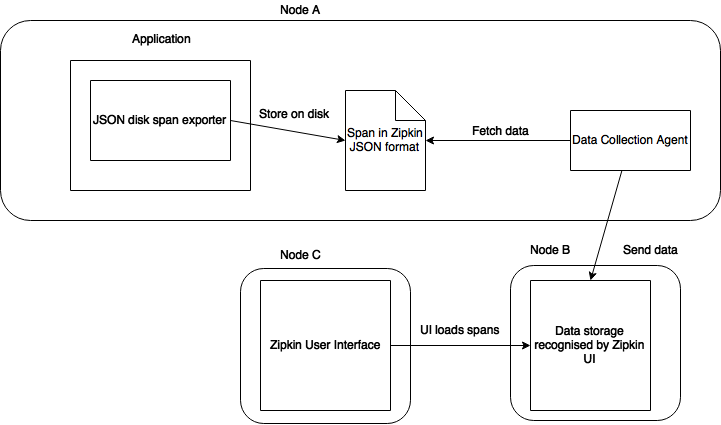
\includegraphics[scale=0.5]{disk_span_exporter.png}
		\caption{Using the JSON disk exporter together with the data collection agent together with the Zipkin user interface .}
		\label{fig:disk_span_exporter}
	\end{figure}
\end{itemize}
Additionally, the Figure \ref{fig:custom_span_exporter} shows how a custom span exporter may be used.

\begin{figure}
	\centering
	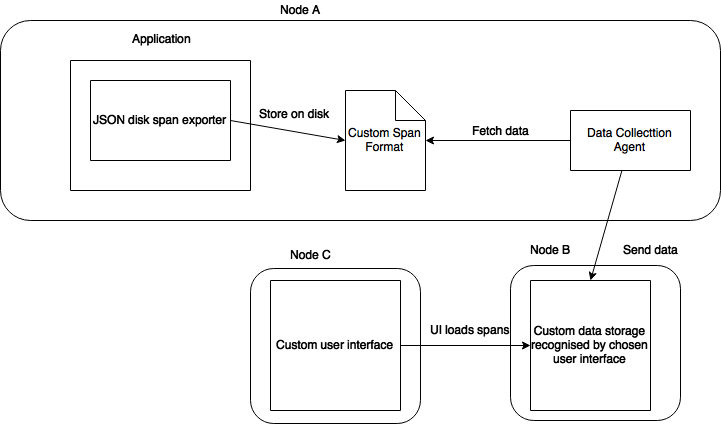
\includegraphics[scale=0.5]{custom_span_exporter.png}
	\caption{Using custom span exporter together with the data collection agent and custom user interface.}
	\label{fig:custom_span_exporter}
\end{figure}

In order to give the developer the flexibility to add new exporters without changing the internals, the custom service loader is used and the span exporters have to be registered in the META-INF directory of the extended instrumentation server JAR file. This ensures that the service loader can find all implementations of the \texttt{SpanExporter} abstract class. The reason why the classes need to be discoverable by the service loader is explained in the Section \ref{desing:native_initialization}.

To make the developer life easier, the \textbf{AutoService} library\footnote{The AutoService library is available at \url{https://github.com/google}.} may used when extending the core server library. Instead of manually registering implementations of custom span exporters into META-INF directory, they can be annotated in the code using the \texttt{AutoService} annotation. This annotation takes a single argument specifying the abstract parent, in this case \texttt{SpanExporter}. The library takes care of registering the classes automatically in the desired folder in correct format so the human error is minimized.

\subsection{Trace Context API}
\label{imp:trace_context_api}
The following methods can be used for obtaining and attaching the trace context:
\begin{itemize}
	\item \texttt{static create()} - creates a new trace context.
	\item \texttt{static getFromObject(holder)} - gets the existing trace context from the holder object.
	\item \texttt{static getFromThread(thread)} - gets the existing trace context from the specified thread.
	\item \texttt{static getFromCurrentThread()} -  gets the existing trace context from the current thread.
	\item \texttt{attachOnObject(holder)} - attaches the trace context to the holder object.
	\item \texttt{attachOnThread(thread)} - attaches the trace context to the specified \newline thread.
	\item \texttt{attachOnCurrentThread()} - attaches the trace context to the current \newline thread.
	\item \texttt{deepCopy} - creates a deep copy of the trace context. It is usually used in cases where child spans are processes in parallel by multiple threads. In this case, the copy of trace context with the same id is shared among all these threads, but they operate on very own objects. This is done in order to allow monitoring of parallel spans within a single trace without having to face race conditions on a single trace context object.
\end{itemize}

The methods above can also be chained and, for example, a trace context can be obtained from the holder object, deep copy created and the newly created copy attached to a new holder object.


\section{Native Agent}
This section covers specific parts of the native agent in more detail. It starts with explanation of considered approaches for instrumentation during the development. The problem of instrumentation server requiring the dependencies for each instrumented class is explained together with the problem of instrumenting the classes with cyclic dependencies. The final solution is explain as well. Further, the instrumentation API, which is used for communication with the server, is explained. Last section describes the byte code parsing.
\subsection{Instrumentation Details}
\label{imp:native:inst}
The native agent does not perform the instrumentation, but asks the server to carry out the transformation. The agent obtains the original bytecode for the class, sends the bytecode to the instrumentation server, waits for the transformed bytecode and lastly, applies the instrumented bytecode.

The instrumentation server requires all dependencies to be available for the the class currently being instrumented. This means that all other classes referenced inside the class file need to be available on the instrumentation server. This includes:
\begin{itemize}
	\item Argument types of all methods.
	\item Return type of all methods.
	\item Type of all fields.
	\item Type of a super class.
	\item Type of implemented interfaces.
\end{itemize}
The dependencies have to be loaded also for the referenced types. To achieve this, we tried two solutions, but only the second solution shown to be feasible.

\subsubsection{Unsuccessful Solution}
The first and unsuccessful solution was based on the fact that several \texttt{Class File load Hook} callbacks may be executed multiple times in different threads. When the application loads a class, the \texttt{Class File load Hook} event is triggered and bytecode ot this class is made available. In this method, the new \texttt{Class File load Hook} event was artificially enforced via the \texttt{RetransformClasses} JVMTI method. This method accepts array of classes for which the hook should be re-thrown. In order to continue with the instrumentation of the original class, all dependent classes have to be instrumented first. However, the classes with cyclic dependencies are not supported in this approach In order to instrumented a class with some cyclic references, all dependencies have to be instrumented first, which is also the class itself.

This solution faced also a different problem. Since the number of dependencies can be significant, the problem of too many threads being opened at a single time has also appeared. 

\subsubsection{Chosen Solution}
The second and currently used solution is based on the fact that Java class files may be accessed as a resource using the class loader, which is loading the class. The class file can be accessed using the \texttt{getResourceAsStream} method. In this solution, the instrumentation server is first asked whether the class currently being loaded should be instrumented. If the class is marked for instrumentation, its bytecode is sent to the instrumentation server\footnote{This step is done only in case if the bytecode for the class is not already available}. Then, all references are scanned in the class file. For this, we need to parse the raw JVM bytecode. More details about this process is explained in the Section \ref{imp:parsing}. Loading of dependent classes is recursively called for each references class until the class does not have any other dependencies, or if all the dependencies are already uploaded on the instrumentation server. Once all dependencies for the class have been sent to the server, the instrumentation process is started and the agent waits for the transformed bytecode. 

Disadvantage of this solution is that developers may override this method in their applications and not provide access to the class files. This is a limitation of the thesis. However, when a such event happens, the instrumentation does not end with the exception, but the attempt to load the class using a different class loader created artificially is done. 

\subsubsection{Initializers and Interceptors}
The instrumentation library used at the server (Byte Buddy) is using so called \texttt{Initializer} class to set up special interceptor field in the instrumented classes. It is a static field, which references the instance of the class interceptor. An interceptor is a class, which defines the instrumentation code. This interceptor field is automatically set by Byte Buddy framework using the corresponding initializers in most use-case of this library. However, in case of the Distrace tool, the instrumentation is performed in different JVM then where the code is actually running and Byte Buddy can't handle this case automatically. Therefore, setting of the interceptor field has to be handled explicitly.

In order to set this field by corresponding initializer, both the initializer class and interceptor class need to be available on the agent. The instrumentation server sends the initializer class together with the instance of interceptor during the instrumentation of the class. Upon receiving, the agent registers the interceptor and initializers with the instrumented class for later to be applied. The interceptor field is static and can be set up only when the class is used for the first time. Therefore, the initializers are loaded during \texttt{Class Prepare} event triggered by the JVM with the application and set up the interceptor field of the class. This event is triggered when the class is prepared, but no code has been execute so far. 

This is not required in case the Advice API is used for the instrumentation. More information about the Advice API is in the Section \ref{back:code_transform}.

\subsection{Auxiliary Classes}
Auxiliary classes are created at run-time during the instrumentation of a class by Byte Buddy framework. The developer can annotate the class to be instrumented with Byte Buddy annotations. These annotations tell the framework to create for example a proxy to a super class or proxy classes to fields of the instrumented class. These proxies then can be used inside the instrumented code to access the objects outside the scope of the instrumented method. Any instrumented class, which is using these auxiliary classes, requires them to be available at run-time on the JVM with the application. Therefore, the native agent asks the server  during the instrumentation for bytecode of the auxiliary class associated to the currently instrumented class. After receiving, the native agent saves the bytecode as a Java class file on disk and makes the class available to the application by adding the class on the application's classpath.

\subsection{Instrumentation API}
The \texttt{Instrumentation API} provides several methods used internally to communicate with the instrumentation server. It defines low-level methods for sending data in form of byte arrays or strings and the corresponding methods for receiving the data. Several more complex methods are built on top of these basic ones to make the communication easier. The most important methods are in the API are:
\begin{itemize}
	\item \texttt{sendClassData} - sends bytecode to the instrumentation server.
	\item \texttt{isClassOnInstrumentor} - checks, whether the bytecode for a given class is already available on the instrumentation server.
	\item \texttt{instrument} - triggers the instrumentation and returns the instrumented bytecode.
	\item \texttt{loadInitializersFor} - loads initializers for a specific class.
	\item \texttt{loadDependencies} - loads all dependent classes and sends them to the instrumentation server.  A dependent class is uploaded only in case it's not already available on the instrumentation server.
	\item \texttt{shouldContinue} - checks if the class on its input is marked for the instrumentation.
	\item \texttt{loadPrepClasses} - loads all classes, which are required by the monitoring tool to be available at run-time on the JVM with the application. These are for example \texttt{TraceContext} and \texttt{Span} classes.
\end{itemize}

\subsection{Byte Code Parsing}
\label{imp:parsing}
Byte code parsing is necessary feature of the Distrace tool and is required for discovering the list of all dependent classes of a class currently being loaded. No sufficient C++ implementation has been found and therefore, a custom parsing module has been implemented. Byte code parsing module in the Distrace tool is inspired by the Apache Commons BCEL library\footnote{More information about this library can be found at \url{https://commons.apache.org/proper/commons-bcel/}.} written in Java. We created very simplified C++ equivalent of this library with features required for our needs.

The main entry point for parsing is the \texttt{ClassParser} class, which contains \texttt{parse} method accepting the bytecode of a class to be parsed. The \texttt{ClassParser} class also defines several accessors for the parsed information. For example, we can get name of the super class name, list of all implemented interfaces, list of all methods or list of all defined fields and their types.

The bytecode structure consists of several parts:
\begin{itemize}
	\item \textbf{Magic id} - Magic id is the first integer stored in each bytecode and is always set to 0xCAFEBABE hexadecimal number.
	\item \textbf{Version} - Version consist of two numbers of \texttt{short} type. The first short represents minor Java version and the second major Java version.
	\item \textbf{Constant pool} - Constant pool is a table, which contains mapping from id, representing a Java type, to the fully qualified type name. Id can represent interface names, field names and also other important constants.
	\item \textbf{Class Info} - Class Info contains the information whether the currently parsed bytecode represents a class or an interface. It also contains name of this class and name of the parent class.
	\item \textbf{Interfaces} - This part of bytecode contains the number of interfaces this class implements. This number is followed by id of type \texttt{short} for each interface. The fully qualified name of an interface can be looked up using the class pool.
	\item \textbf{Fields}. This part of the bytecode contains the number of fields this class defines together with some additional information for each defined field. The fully qualified type of a field can be looked up using the class pool.
	\item \textbf{Methods}. This part contains the number of defined methods in the bytecode together with some additional information for each method such as the number of arguments. The fully qualified types of return value and arguments of the method can be looked up using the class pool.
\end{itemize}
More information about the class file structure can be found at the official Java documentation\footnote{The documentation of the class loading process is available at \url{https://docs.oracle.com/javase/specs/jvms/se7/html/jvms-4.html}.}.
Each section of a class file is parsed separately. \texttt{ByteReader} class is used as a reader of the raw bytecode and contains several methods for reading different types of data from the bytecode array. 

Parsing the magic id and both, minor and major versions, is straightforward as they are just numbers and can be read using the \texttt{ByteReader} class directly. Parsing of the constant pool is more complex. For each entry in the constant pool a constant representing the entry is read. Each constant represent a specific object. For example a constant can represent a class, string, type of a field or return value and arguments of a method. Once the constant pool is parsed, it can be queried for the specific symbols using their id. Class name, super class name, interfaces, fields and methods are read from the constant pool using their ids.

\section{Instrumentation Server}
This section describes several technical parts of the instrumentation server. The details of the instrumentation itself are provided first, followed by an overview of the optimizations the server does to speed up the communication with the native agent. The next sections describes how trace context is injected to instrumented classes and how native methods at Java are bound to their implementations on the native agent side. The last section describes how JSON objects, which represent spans, are generated.

\subsection{Instrumentation Details}
\label{impl:server:instr}
The classes to be instrumented are marked using the \texttt{MainAgentBuilder} and \texttt{BaseAgentBuilder} classes.
The instrumentation server expects the instance of \texttt{MainAgentBuilder} on the input of its \texttt{start} method. This builder is the abstract class containing single abstract method \texttt{createAgent(BaseAgentBuilder builder, String pathToHelperClasses)}, where the builder is a wrapper \linebreak around the Byte Buddy \texttt{AgentBuilder} class, which is used to define the class transformers.

The developer extending the core instrumentation server needs to implement this method and specify on which classes and on which methods the instrumentation should happen. Since Byte Buddy is used for writing transformers and interceptors, more information about Byte Buddy library is located in the Section \ref{sec:byte_buddy}. In short, transformers are used to identify the class to be instrumented. They consist of advice or interceptors identifying the particular methods to be instrumented on the given class. The advice and interceptors also contain the code to be injected to the instrumented methods. The server provides several helper methods for creating the transformers and interceptors, which are less verbose then the standard Byte Buddy approaches.

Each interceptor has to implement the \texttt{Interceptor} interface. This is required so the server can discover all interceptor implementations at run-time without the need of changing the internals of the server. Each implementation of the interceptor needs to register itself in the META-INF directory of the generated JAR file in the same way as the span exporters mentioned in the Section \ref{imp:exporter}. Custom service loader is then used to locate all classes implementing the \texttt{Interceptor} interface. The interceptors need to be discovered since the instrumented classes depend on the interceptors and require them at run-time. Therefore, the instrumentation server have to send them to the native agent to make them available to the monitored application.

The advice may be used without any special annotations since Byte Buddy in-lines the code defined by the advice into the original code. Therefore, there is no need to transfer the advice implementations to the monitored application.

Even though Byte Buddy takes care of the internals of the instrumentation, the \texttt{BaseAgentBuilder} class is internally properly configured so the instrumentation is defined exactly as desired. This class implements four Byte Buddy listeners used reporting about the instrumentation progress. These listeners allow us to react on the process of the instrumentation. The listeners are:
\begin{itemize}
	\item \texttt{onTransformation} listener is called immediately before the class is instrumented. Implementation of the listener in the Distrace tool also sends to the agent all auxiliary classes required by the instrumented class and the initializers used for setting the static interceptor field on the instrumented class.
	\item \texttt{onIgnored} listener is called when the class is not marked for instrumentation. The class is not instrumented if the developer does not define any transformer for the specified class.
	\item \texttt{onError} listener is called when some exception occurred during the instrumentation.
	\item \texttt{onComplete} listener is called when instrumentation sucessu completed. It is called after both of \texttt{onTransformation} and \texttt{onIgnored} listeners.
\end{itemize}

Byte buddy requires all dependent classes for the instrumented class to be available. They are needed because the instrumentation framework needs to know signature of all methods so it can correctly identify the methods to be instrumented. The dependencies are all classes referenced in the class file such as type of the method return value and arguments, super class and implemented interfaces. 

By default, Byte Buddy library attempts to find these dependencies using  \texttt{LocationStrategy} and \texttt{PoolStrategy} classes. The first class is used to tell Byte Buddy where to look for the raw bytecode of dependent classes. By default, the classes are loaded by the context class loader, but since the classes to be instrumented are received over the network, custom \texttt{InstrumentorClassloader} class loader is used to handle the class loading. It is a simple class loader which loads the class data from the agent and caches them. When there is a request for instrumentation, instead of looking into the class files, this class loader loads the bytecode from the cache and passes it to the Byte Buddy.

However, Byte Buddy internal API does not work directly with raw bytecode. It uses classes \texttt{TypeDescription} and \texttt{PoolStrategy}. The first class has a constructor accepting the \texttt{Class} class. The  instance of this class contains metadata for the class passed to the constructor, such as the signature of all methods and fields, list of all interfaces or for example list of constructors. The second class is used for caching the type descriptions so they are not created every time the class is accessed. 

In overall, class lookup is done in the following two steps:
\begin{enumerate}
	\item Check whether type description for the class is available. If yes, load the type description from the cache.
	\item If the type description is not available, load the class using the \linebreak \texttt{InstrumentorClassloader}, create type description for the class and put it in the cache.
\end{enumerate}

\subsection{Optimizations}
The instrumentation server performs several optimizations to speed the communication with the native agent. The first optimization is caching of the classes sent to the instrumentation server from the native agent and also caching of already instrumented classes. This behavior is useful in cases where the native agents are sharing the instrumentation server. When a class is received from any agent, it is cached and the rest of the agents don't need to send the original class again when they request the instrumentation from the server. The server also performs the instrumentation only once and caches the instrumented classes. When any agent queries the server to instrument already instrumented class, the server can send the class immediately from the cache.

The second way how the communication can be optimized is influenced by the user. The user may compile the extended instrumentation server with the application classes or add these classes on the classpath of the server. When a native agent asks the server for instrumentation of a class, the server first check if it can load the class locally and avoid transferring the bytecode from the native agent. 


\subsection{Span Injection}
This short section explains how span and trace details are internally attached to the instrumented classes. The trace information is attached to the class by adding a new synthetic field with name \texttt{\_\_\_\_traceContext}. This trace context represents the current trace and is used in the code to obtain reference to a current trace context and also current span. This new field is created using the Byte Buddy instrumentation builder with the \texttt{defineField} method.


\subsection{Binding the Native Methods}
This section explains how methods implemented on the native agent can  be used in the classes defined on the instrumentation server. Some classes created at the instrumentation server, such as \textbf{SpanExporter} class, have to use data from the native agent. This is achieved by creating a helper method at the agent side, which returns the required data, and by creating corresponding native method on the Java side. When a class, which defines these native methods, is sent to the native agent and used for the first time, the native method in Java is bound to the implementation in C++. The methods are bound together inside the callback for the \texttt{Prepare} event. This ensures that we can define native methods in Java and bind them with their implementations on the separated machine, in this case the machine with the native agent. Also, this can have performance benefits, since these methods are written as native methods.

For example, this technique is used for accessing the span exporter type inside the \texttt{SpanExporter} abstract class. This class is defined at the instrumentation server, however the exporter type is passed as an argument to the native agent. This class contains the native method named \texttt{getSpanExporterType}, which returns the span exporter type. The \texttt{SpanExporter} class is sent to the native agent during the agent initialization and when it's used for the first time, the \texttt{getSpanExporterType} method is bound to the corresponding C++ implementation, which provides value of this argument.

\subsection{JSON Generation}
\label{json_gen}

The collected data inside spans are internally stored as instances of \texttt{JSONValue} class representing any JSON value. JSON format is chosen since default Zipkin user interface expects spans in this format. JSON is a lightweight format for exchanging data with the syntax based on Javascript object notation.

The JSON handling is inspired by the minimal-json library\footnote{The library is available at \url{https://github.com/ralfstx/minimal-json}.}. The simplified custom implementation was created which provides features required by the Distrace tool. Also the number of dependencies required to build is tool is lowered since this code is part of the Distrace sources.

This JSON support is designed via several classes:
\begin{enumerate}
	\item \textbf{JSONValue} - The abstract ancestor for all JSON types. This type defines common methods to all implementation.
	\item \textbf{JSONString} - A class representing string types.
	\item \textbf{JSONNumber} - A class representing numeric types.
	\item \textbf{JSONLiteral} - A class representing the literals \textbf{null}, \textbf{true} and \textbf{false}.
	\item \textbf{JSONArray} - A class representing the JSON arrays. It has support for adding new elements into the array.
	\item \textbf{JSONObject} - A class representing the JSON objects. It has support for adding a new items into the object.
\end{enumerate}

Each \textbf{JSONValue} can be exported as string where the printing is driven by the \texttt{JSONStringBuilder} class. This class is also responsible for escaping the characters according to JSON standards. The default printer exports the data without any formatting into a single text line, however \texttt{JSONPrettyStringBuilder} exports the data in more human-readable format. The second printer is usually used for the debugging purposes and the first one is used for exporting spans in real scenario as the size of the data is smaller in this case.


